% !TeX spellcheck = en_US
\chapter{Evaluation}\label{ch:evaluation}

This chapter is about the evaluation of the several approaches presented in Ch.~\ref{ch:approach} and~\ref{ch:implementation}.

\section{Experimental Setup}

For the following evaluations HDT-Java 2.0~\footnote{\label{foot:1}https://github.com/rdfhdt/hdt-java/releases/tag/v2.0} (the currently newest version) has been used. For GRP the implementation presented in Ch.~\ref{sec:relatedworkGRPImpl} has been used.

\section{GRP vs HDT}\label{sec:evaluationHDTvsGRP}

\todo{passt alles nicht mehr wegen neuer Erkenntnis}

Fig.~\ref{fig:ratiosHDTWithoutDict} shows $CR_{Graph_{HDT}}$. As expected, $CR_{Graph_{HDT}}$ gets higher the more similar the graph is to the authority pattern. In general it can be said that this effect is quite small. There is only a distance of 0.002 between the minimum and the maximum. This small effect can also be seen by looking at Fig.~\ref{fig:ratiosHDTWithDict}. It can be seen that the size of the dictionary ($out_{dict}$) has a much bigger effect, since $CR_{HDT}(out)$ is much larger than $CR_{Graph_{HDT}}$ and the curve behavior from Fig.~\ref{fig:ratiosHDTWithoutDict} is no longer recognizable. It is noticeable that $|out_{dict}|$ is bigger when the graph is further away from the star pattern. $Dict_{HDT}$ seems to be more inefficient when there are about as many subject as objects. 

\begin{figure}[h]
	\centering
	\subfloat[$CR_{Graph_{HDT}}$.]{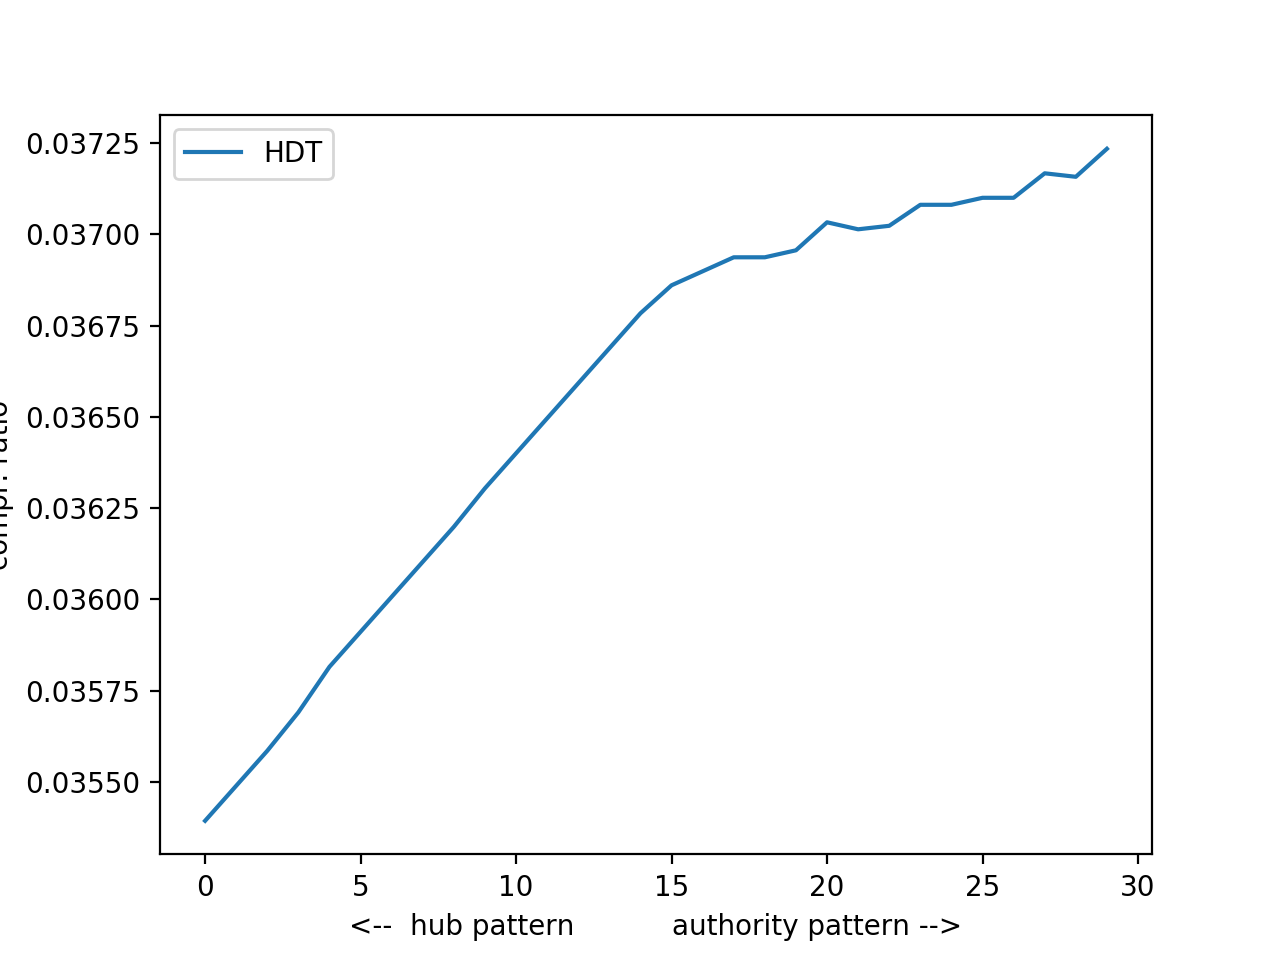
\includegraphics[width=0.5\textwidth]{figures/GRPvsHDT/hdtWithoutDict}\label{fig:ratiosHDTWithoutDict}}
	\hfill
	\subfloat[$CR_{HDT}$.]{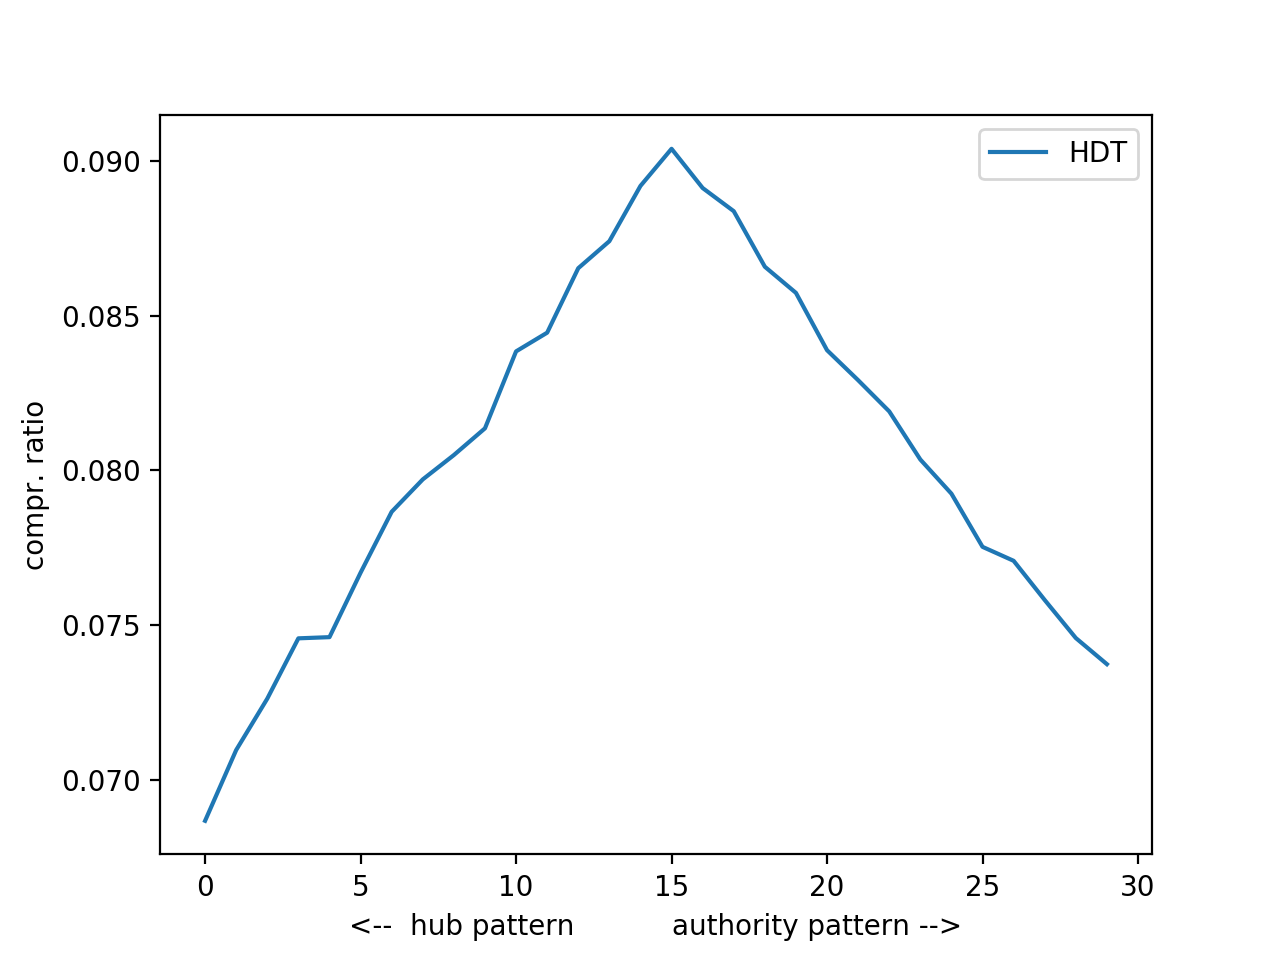
\includegraphics[width=0.5\textwidth]{figures/GRPvsHDT/hdtWithDict}\label{fig:ratiosHDTWithDict}}
	\caption{The compression ratios for HDT without and with dictionary sizes.}
\end{figure}

Next, the compression ratio of GRP ($CR_{Graph_{GRP}}$) is considered, which is presented in Fig.~\ref{fig:ratiosGRPWithoutDict}. Here, it is noticeable that GRP has a better compression ratio if the graph is more similar to the star pattern (hub or authority pattern). This property of GRP has also been mentioned in~\cite{maneth}. It can also be seen that the effect is higher on $CR_{Graph_{GRP}}$ than on  $CR_{Graph_{HDT}}$ (standard deviation is twice as high for $CR_{Graph_{GRP}}$ as for $CR_{Graph_{HDT}}$). 

When Fig.~\ref{fig:ratiosGRPWithDict} is considered, it can be seen that this curve behaves almost exactly like the one from Fig.~\ref{fig:ratiosHDTWithDict}, since $|out_{dict}|$ accounts for most of $|out|$.

\begin{figure}[h]
	\centering
	\subfloat[$CR_{Graph_{GRP}}$.]{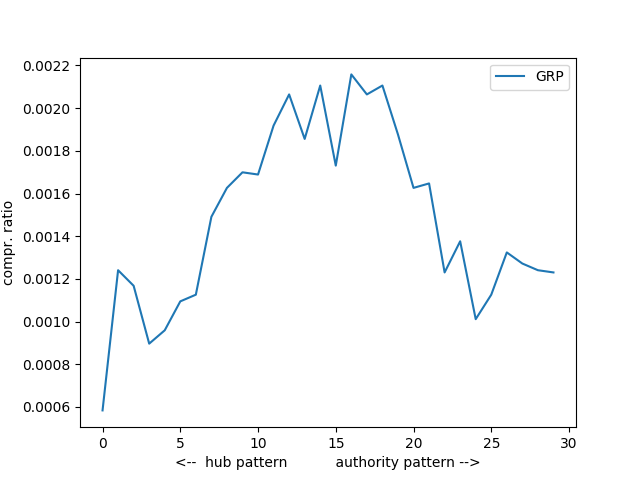
\includegraphics[width=0.5\textwidth]{figures/GRPvsHDT/grpWithoutDict}\label{fig:ratiosGRPWithoutDict}}
	\hfill
	\subfloat[$CR_{GRP}$.]{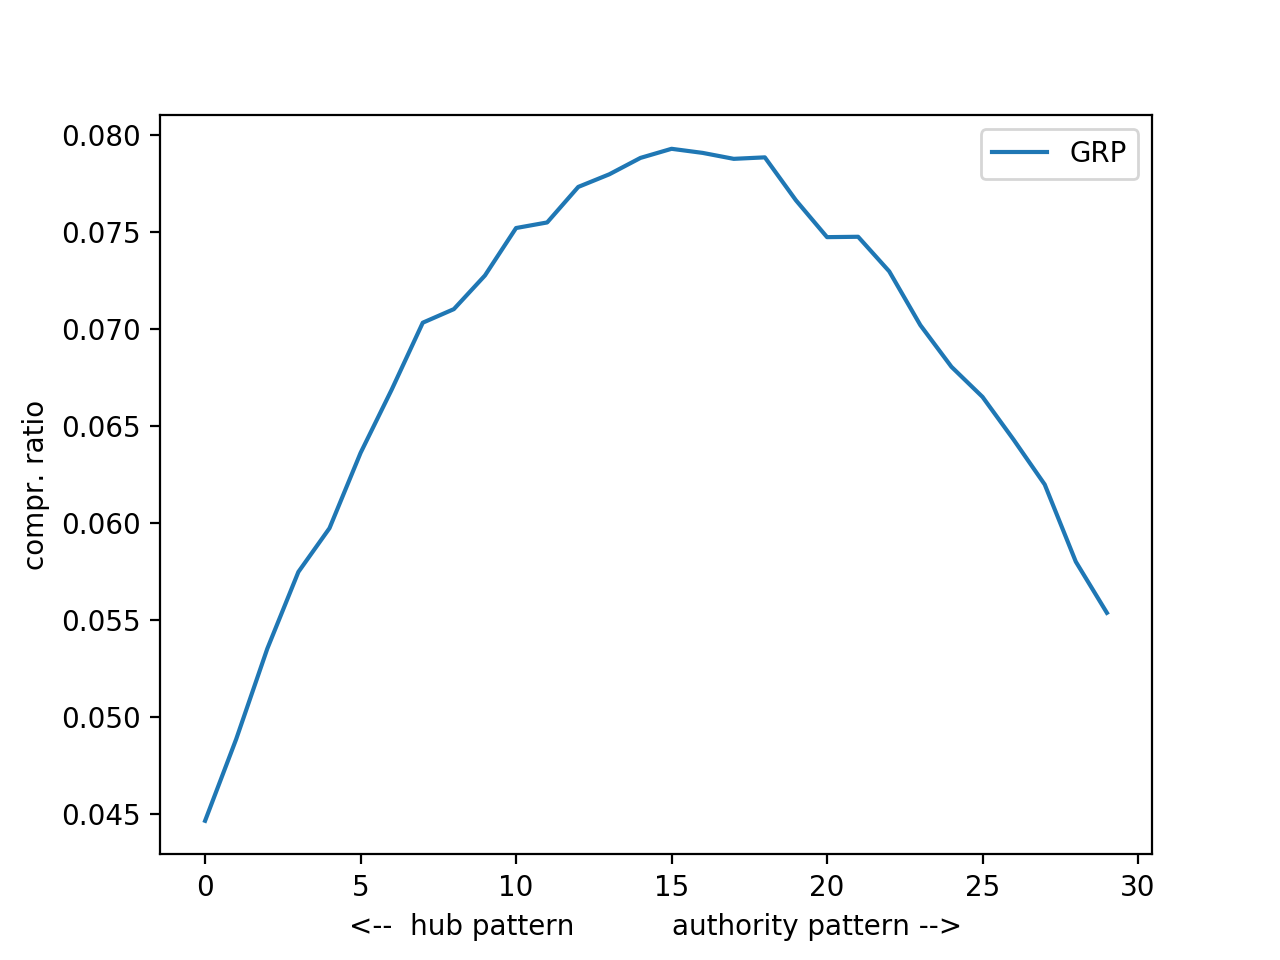
\includegraphics[width=0.5\textwidth]{figures/GRPvsHDT/grpWithDict}\label{fig:ratiosGRPWithDict}}
	\caption{The compression ratios for GRP without and with dictionary sizes.}
\end{figure}

Finally, Fig.~\ref{fig:ratiosBothWithoutDict} and Fig.~\ref{fig:ratiosBothWithDict} show $CR_{Graph_C}$ and $CR_C$, respectively for GRP and HDT. Since both use $Dict_{HDT}$ to compress the dictionary, the curves in Fig.~\ref{fig:ratiosBothWithDict} are very similar. However, it becomes clear that GRP compresses better than HDT. In Fig.~\ref{fig:ratiosBothWithoutDict}, $CR_{Graph_{HDT}}$ is 31 times higher than $CR_{Graph_{GRP}}$ on average. Of course, this factor becomes much smaller in Fig.~\ref{fig:ratiosBothWithDict} because the dictionary accounts for most of the memory size. Here, the $CR_{HDT}$ is on average 1.8 times as high as $CR_{GRP}$

\begin{figure}[h]
	\centering
	\subfloat[$CR_{Graph_{HDT}}$ and $CR_{Graph_{GRP}}$.]{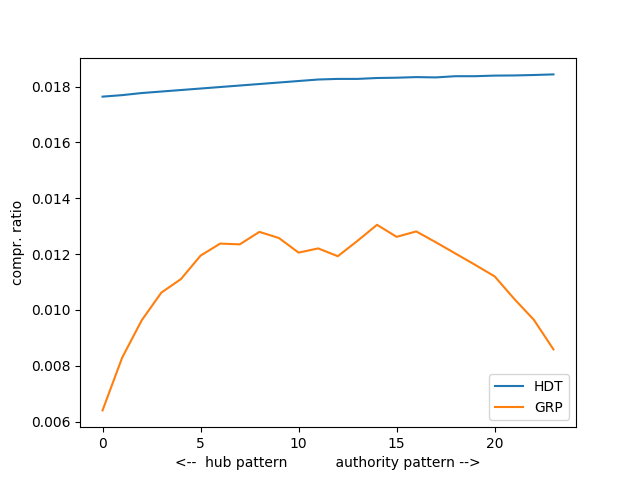
\includegraphics[width=0.5\textwidth]{figures/GRPvsHDT/bothWithoutDict}\label{fig:ratiosBothWithoutDict}}
	\hfill 
	\subfloat[$CR_{HDT}$ and $CR_{GRP}$.]{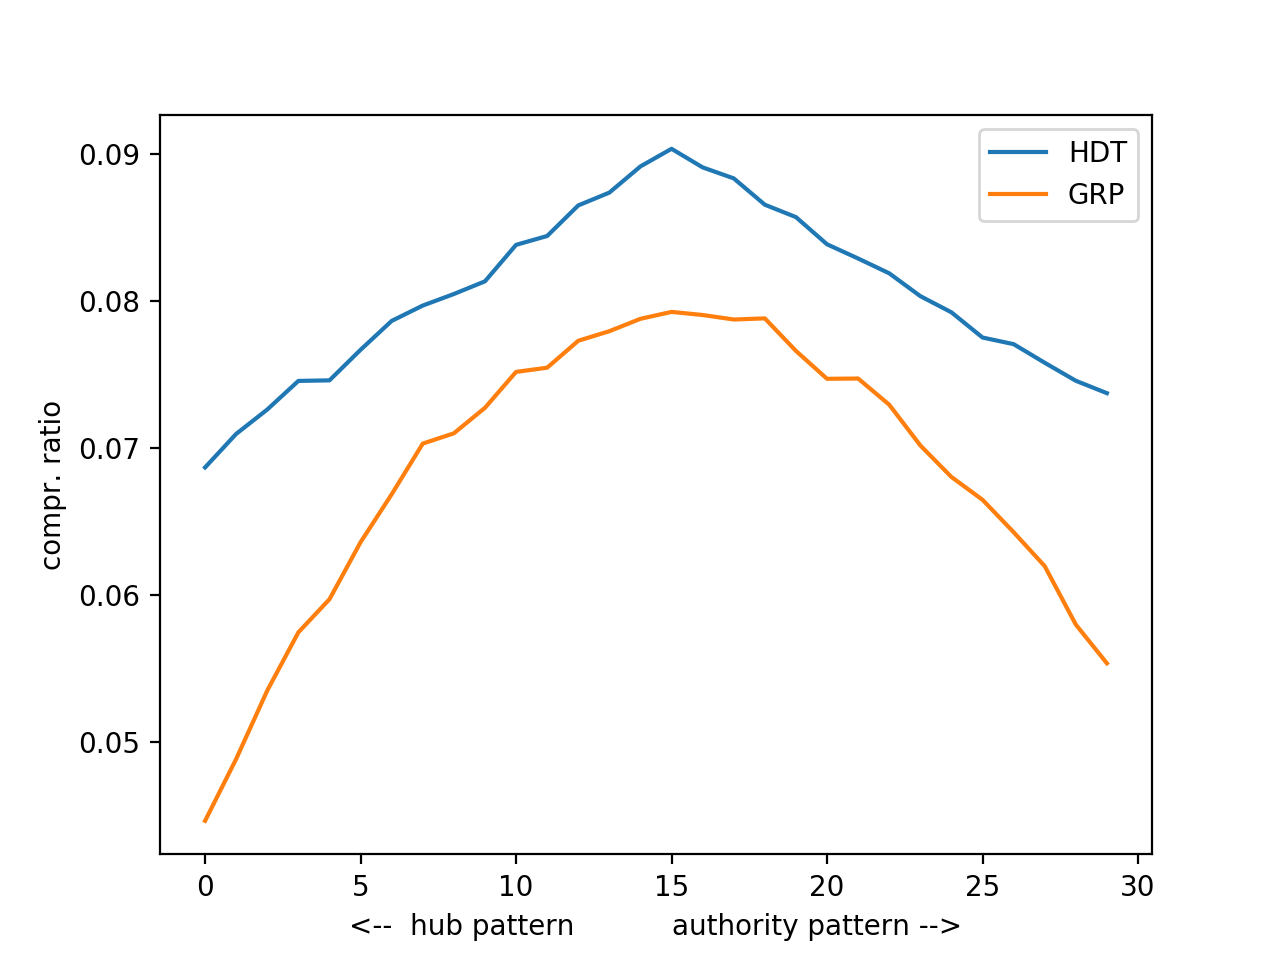
\includegraphics[width=0.5\textwidth]{figures/GRPvsHDT/bothWithDict}\label{fig:ratiosBothWithDict}}
	\caption{The compression ratios for GRP and HDT without and with dictionary sizes.}
\end{figure}

It would be possible to argue that only one distinct predicate was used in that scenario and this is beneficial for GRP, as it gets worse as the number of predicates increases. Therefore a further evaluation is made in Fig.~\ref{fig:bothwithdict1000predicates}, where 1000 distinct predicates have been used. That is a quite high number considering the number of triples (1199) compared to real RDF data \todo{belegen}. It is visible that the compression ratios are now higher for both compressors, but still $CR_{GRP}$ is always smaller than $CR_{HDT}$. $CR_{HDT}$ is still 1.7 times higher on average. So, the increasing number of predicates has a similar effect on both algorithms.


\todo{figure passt nicht}
\begin{figure}
	\centering
	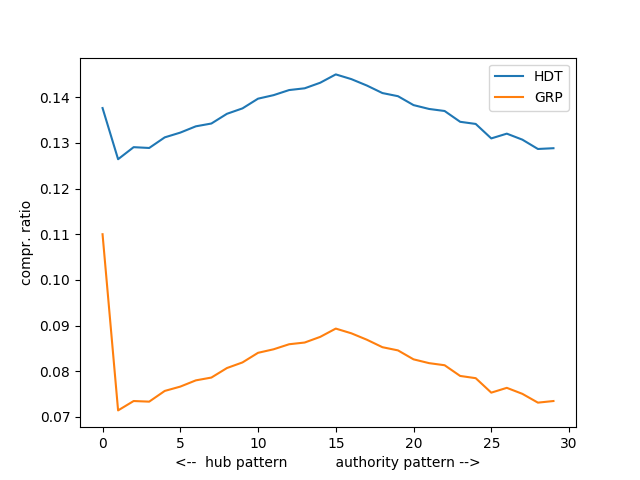
\includegraphics[width=0.7\linewidth]{figures/GRPvsHDT/bothWithDict1000Predicates}
	\caption{$CR_{HDT}$ and $CR_{GRP}$. Graphs have now 1000 distinct predicates.}
	\label{fig:bothwithdict1000predicates}
\end{figure}

Apart from the compression ratio, the run time is also important for the overall performance. Fig.~\ref{fig:runtimes} shows the average value of $CT$ for both compressors, respectively. For this the same scenario with the star pattern (and only one distinct predicate) was used. It has been executed 100 times to get a sophisticated run time measurement, because $CT$ depends on the current CPU workload of the computer.

\begin{figure}
	\centering
	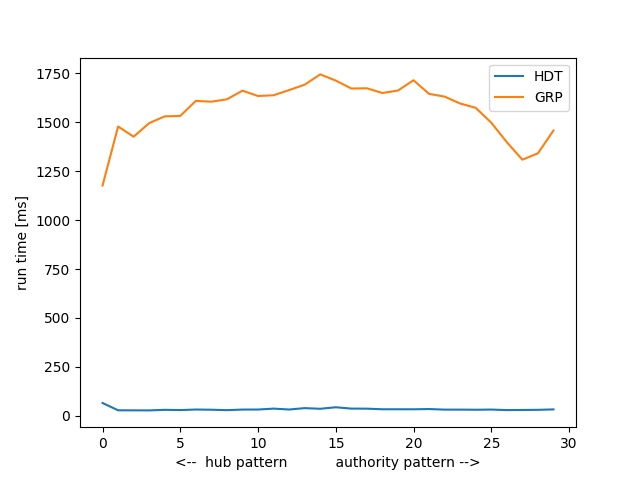
\includegraphics[width=0.7\linewidth]{figures/GRPvsHDT/runtimes}
	\caption{$CT_{HDT}$ and $CT_{GRP}$ (Average run time of 100 consecutive executions).}
	\label{fig:runtimes}
\end{figure}


It can be seen that $CT_{GRP}$ is significantly higher than $CT_{HDT}$. It is on average ca. 48 times as high.

However, it should also be noted that the implementation of GRP is rather rudimentary  (according to the authors of~\cite{maneth}), while that of HDT has been under development for some time. So they are not comparable in terms of quality. Unfortunately, it is not possible say at this point whether a more professional implementation of GRP will also be slower than HDT.

In addition it can be noticed that $CT_{GRP}$ fluctuates more than $CT_{HDT}$. $CT_{GRP}$ has a standard deviation of about 134, while $CT_{HDT}$ only has a standard deviation of about 7. One reason for this is that GRP, in contrast to HDT, is non-deterministic because of the partly random search order of the graph. On the other hand, the high deviations are also a confirmation of the above mentioned hypothesis that the behavior of GRP depends more on the structure of the input data than HDT does.



\section{Compression Improvements}

This chapter is about evaluating the compression improvements. It starts with applying ontology knowledge and then continues with dictionary compression improvement. In contrast to Ch.~\ref{sec:evaluationHDTvsGRP}, real data will be evaluated here to see how much influence the improvements have.

\subsection{Ontology Knowledge}\label{sec:evaluationOntKnowledge}

In this chapter, it will be evaluated whether using meta data from the ontology can result in a better compression ratio for $Graph_{GRP}$. 

Here, not only the size of the output $out_{graph}$ will be measured. Since these approaches have the intention to improve the ability for GRP to produce a smaller grammar, the features of that grammar will be presented in more detail. That is because after the encoding of the grammar it might happen that despite the fact that the grammar is smaller after the manipulations that effect is not visible in the value of $|out_{graph}|$. 

\subsubsection{Occurrence of Properties}
Now, it will be presented how much of those symmetric/inverse/transitive properties exist in real data. For that we will use the datasets presented in Ch.~\ref{sec:implementationDatasets}. 

Fig.~\ref{fig:ontoccurrences} shows how often the relevant properties occur in real datasets (DBPedia and Wordnet). (Relative amount = $\frac{\text{number of occurrences}}{\text{number of triples}}$). It can be noticed that the amounts are quite low, especially for symmetric and inverse properties. This supports the hypothesis from Ch.~\ref{sec:implementationOntKnowledge} that building sub graphs with higher amounts of relevant properties can be necessary to observe a real effect of the data manipulations. Nevertheless, first the normal datasets will be used to evaluate the manipulations.

\begin{figure}
	\centering
	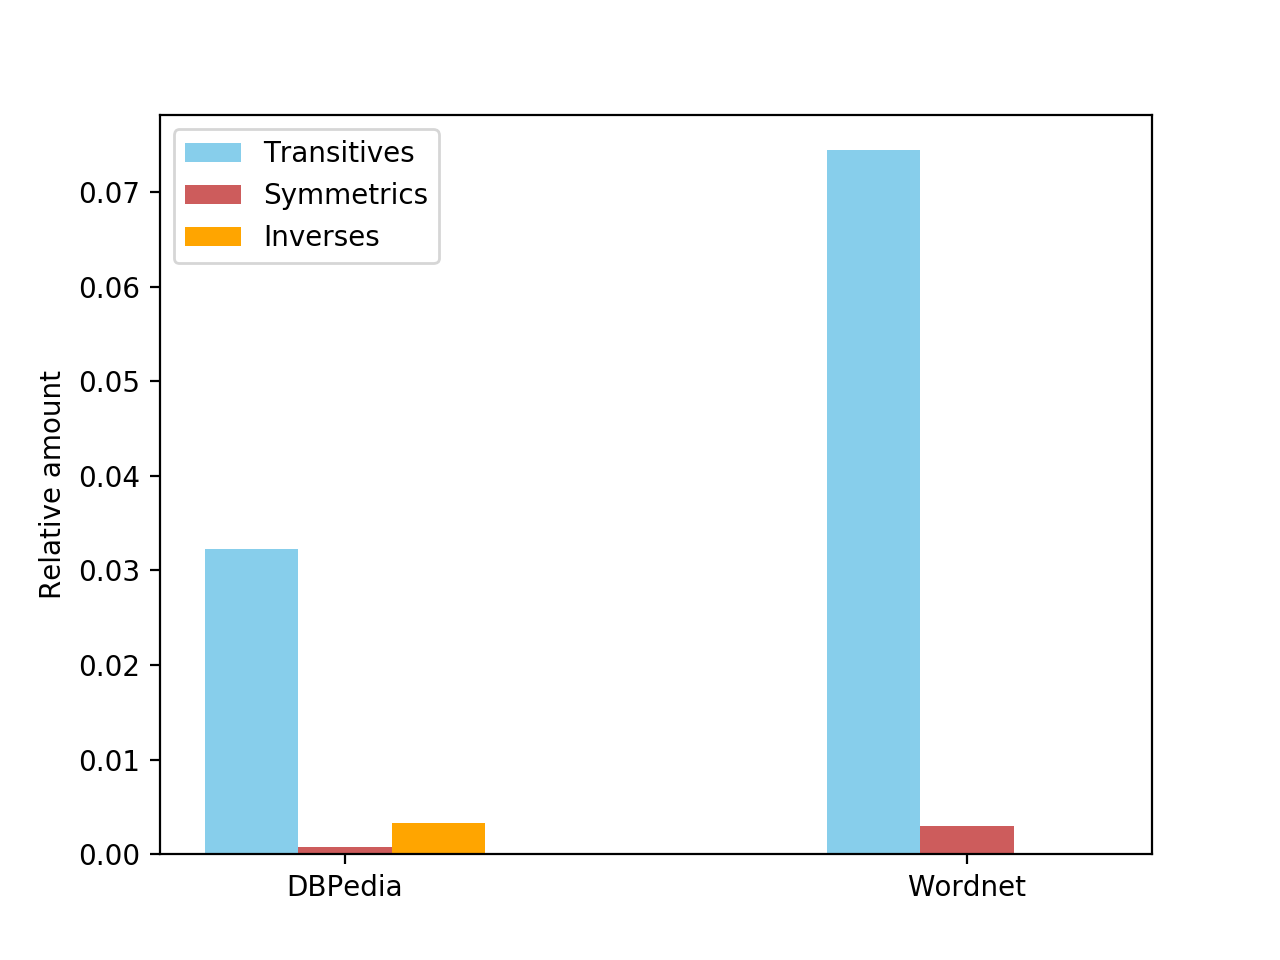
\includegraphics[width=0.7\linewidth]{figures/4_evaluation/ontOccurrences}
	\caption{Relative amount of transitive/symmetric/inverse properties in real datasets.}
	\label{fig:ontoccurrences}
\end{figure}

\todo{irgendiwe zeigen, dass interessante Fälle zu selten auftreten}

Therefore, for the following evaluations of Ch.~\ref{sec:evaluationOntKnowledge}, we use sub graphs as described in Ch.~\ref{sec:implementationSubGraphs}. More precisely, we use graphs that contain half triples with the relevant properties and the other half triples connected with them. By doing that, the effects will be significant and it will be clear whether they lead to a better or worse compression ratio. 

\subsubsection{Evaluation Process}
Now, the overall process of applying ontology knowledge and evaluating whether it results in a better compression is explained. The several parts of the process will be discussed in the next sections. Fig.~\ref{fig:overallprocess} shows how it is implemented. First, the original graph or sub graph is given to GRP. That part is called $in_1$ in Fig.~\ref{fig:overallprocess} and it will deliver the first result $out_1$.

In the next step, relevant properties have to be determined and the original graph will be manipulated. Then the manipulated graph is given to GRP. In addition, the relevant ontology triples have to be compressed and stored as well. Otherwise, the original graph could not be restored. Both graphs together are merged together into one graph called $in_2$ which is then compressed by GRP and that delivers $out_2$. 

Finally, $|out_1|$ and $|out_2|$ have to be compared. The next chapter will explain how that is done.

\begin{figure}
	\centering
	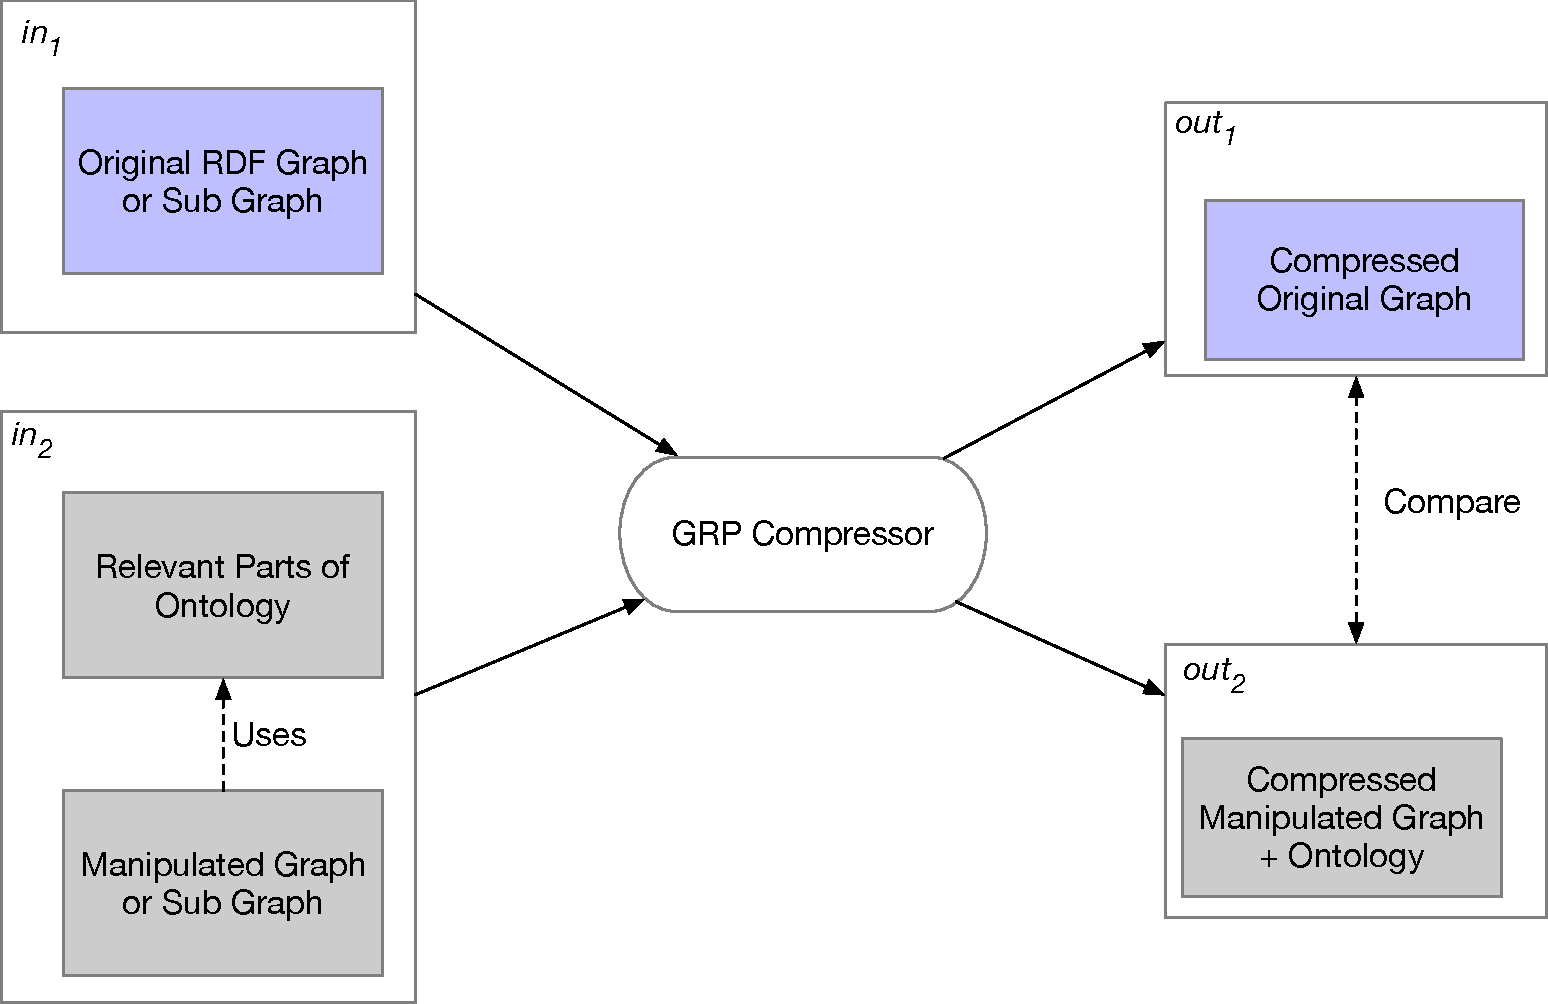
\includegraphics[width=0.9\linewidth]{figures/4_implementation/overallProcess}
	\caption{Overall process of applying ontology knowledge and comparing the compression results.}
	\label{fig:overallprocess}
\end{figure}

The evaluation process must be executed for the different manipulation aspects (symmetric, inverse etc.) independently. So there is one manipulated graph where all symmetric edges are added or removed, and analogously for the other manipulations. Finally, it is also possible to execute the process for one graph in which all different manipulations have been applied. This way, it is noticeable what the manipulations bring individually and in the end also, what they all achieve in combination.\todo{wurde das gemacht?}

\subsubsection{Metrics}

This chapter explains how the two outputs $out_1$ and $out_2$ are compared.

Since the ontology-based manipulations are intended to achieve a better compression by enabling $Graph_{GRP}$ to produce a smaller grammar, it is interesting to not only compare $out_1$ and $out_2$ at the file size level, but also in terms of their grammar/graph sizes. The most significant metric for the size of a grammar/graph is its number of edges. In order to compare $out_1$ and $out_2$ with respect to their grammar/graph edge amounts, the metrics input edge ratio ($IER$) and output edge ratio ($OER$)  are defined:
 
 \[
 IER=\frac {\text{number of edges in } in_2} {\text{number of edges in  } in_1}
 \]
 
 \[
 OER=\frac {\text{number of edges in } out_2} {\text{number of edges in } out_1}
 \]
 
$IER$ shows how many edges have been added or removed by the manipulations which indicates how big the impact of the manipulation is. $OER$  shows whether the manipulation results in a better ($OER<1$) or worse ($OER>1$) compression ratio.

In order to measure the manipulation it is necessary to define a new metric instead of re-using $CR_{GRP}$ as defined in Ch.~\ref{sec:compressorModel}. For $out_1$, $CR_{GRP}$ would be in relation to $in_1$ (analogously for $out_2$ and $in_2$). But here it is necessary to compare $out_1$ and $out_2$. Therefore, the new metric size ratio ($SR$) is defined as follows:

 \[
SR=\frac {|out_2|} {|out_1|}
\]

If $SR<1$ holds than the manipulation has resulted in an improvement at the file size level, otherwise not. Of course, the file size level is in the end more relevant than the grammar level, because it is the real storage amount necessary to store the compressed data.



\subsubsection{Symmetric Properties}

First, the approach suggested in Ch.~\ref{sec:approachOntKnowledge} to add all possible triples with symmetric edges will be evaluated. Fig.~\ref{fig:symmetricAddResults} illustrates the results. Fig.~\ref{fig:edgeratiossymmetricsadd} shows the results on the grammar level, here $IER$ and $OER$ are presented. As expected $IER$ is bigger than 1, as edges have been added to the graph. For both DBPedia and Wordnet $IER$ is about 1.4. The other scale in Fig.~\ref{fig:edgeratiossymmetricsadd} shows $OER$. There, it can be noticed that $OER<1$ holds, which means that adding symmetric triples is indeed beneficial for $Dict_{GRP}$ and even brings a significant improvement on the grammar level as $OER$ is about 0.8 for DBPedia, and about 0.5 for Wordnet.

In Fig.~\ref{fig:sizeratiossymmetricsadd}, $SZ$ is shown. Here, it can be seen that $SR<1$ is true. Hence, also on the file size level the manipulation has delivered a better result. However, the improvement is not as good as on the grammar level. That is because the file \textbf{Perms} (see Ch.~\ref{sec:relatedworkGRPImpl}) becomes bigger in $out_2$, since there are now more hyper edges in the grammar. So, it can be noticed that the encoding algorithm of $Dict_{GRP}$ (see Ch.~\ref{sec:relatedworkGRPImpl}) cannot always take full advantage of a smaller grammar.

\begin{figure}[h]
	\centering
	\subfloat[$IER$ and $OER$]{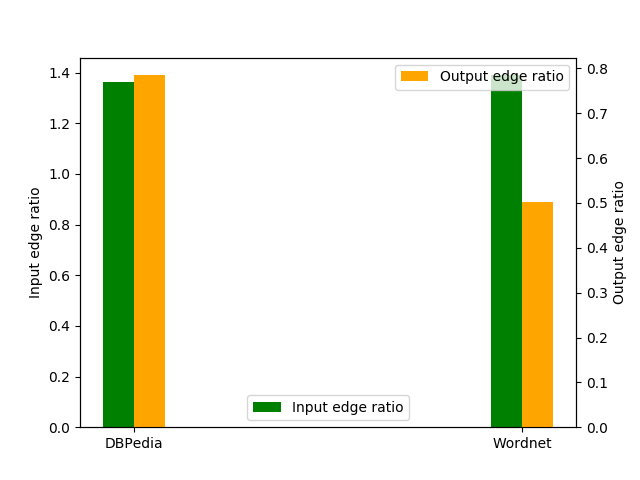
\includegraphics[width=0.5\textwidth]{figures/4_evaluation/ontology/edgeRatiosSymmetricsAdd}\label{fig:edgeratiossymmetricsadd}}
	\hfill 
	\subfloat[$SR$]{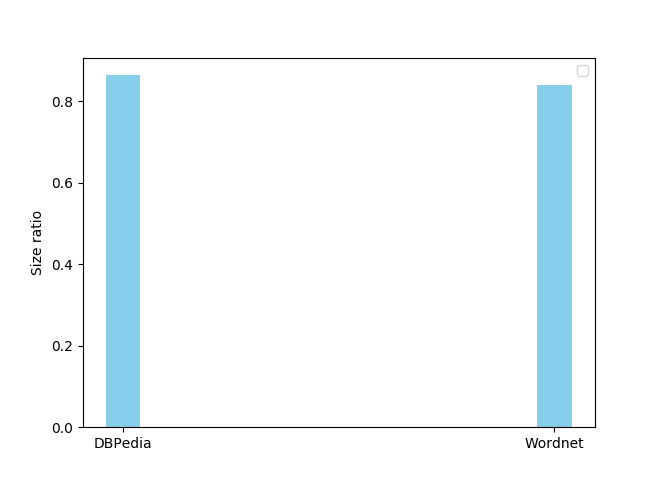
\includegraphics[width=0.5\textwidth]{figures/4_evaluation/ontology/sizeRatiosSymmetricsAdd}\label{fig:sizeratiossymmetricsadd}}
	\caption{Results for adding symmetric properties, on the grammar level (\ref{fig:edgeratiossymmetricsadd}) and on the file size level (\ref{fig:sizeratiossymmetricsadd}).}
	\label{fig:symmetricAddResults}
\end{figure}

In order to show that adding symmetric properties is more beneficial than removing them, the results of the removal case are also shown (see Fig.~\ref{fig:symmetricDeleteResults}). In Fig.~\ref{fig:sizeratiossymmetricsdelete}, it is possible to see that $IER<1$ holds, since edges have been removed. But $IER$ is still quite close to 1, because there are not many cases in which an edge could be removed. Hence, in most cases only one of the two directions for symmetric properties is present in the graph. Both $OER$~(Fig.~\ref{fig:edgeratiossymmetricsdelete}) and $SR$~(Fig.~\ref{fig:sizeratiossymmetricsdelete}) are less than 1, but not less than in Fig.~\ref{fig:symmetricAddResults}, which indicates that adding symmetric edges is more beneficial for $Graph_{GRP}$. However, it can still be argued that there are only a few cases in which edges were removed and that the potentially positive effect is therefore not recognizable.

To further investigate the removal case, the graph $out_2$ from Fig.~\ref{fig:symmetricDeleteResults} is taken as the input $in_1$ for a new evaluation. So, $in_1$ will be an artificial graph in which for each symmetric property only one direction of the triples exist. This extreme case can show whether adding or removing symmetric edges will be better, since $in_1$ is a graph where all symmetric edges have been removed before hand.

\begin{figure}[h]
	\centering
	\subfloat[$IER$ and $OER$]{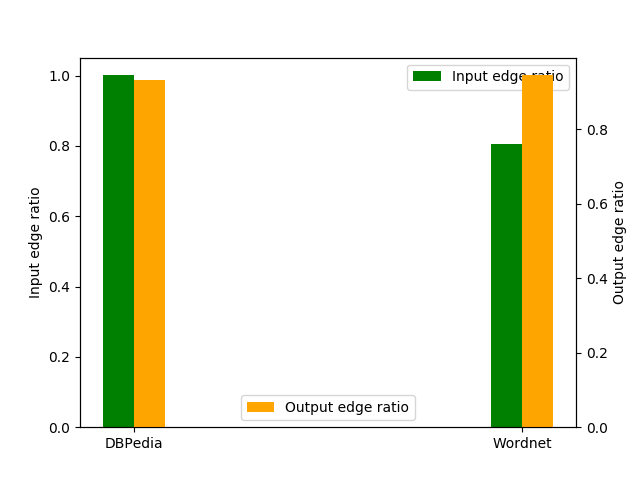
\includegraphics[width=0.5\textwidth]{figures/4_evaluation/ontology/edgeRatiosSymmetricsDelete}\label{fig:edgeratiossymmetricsdelete}}
	\hfill 
	\subfloat[$SR$]{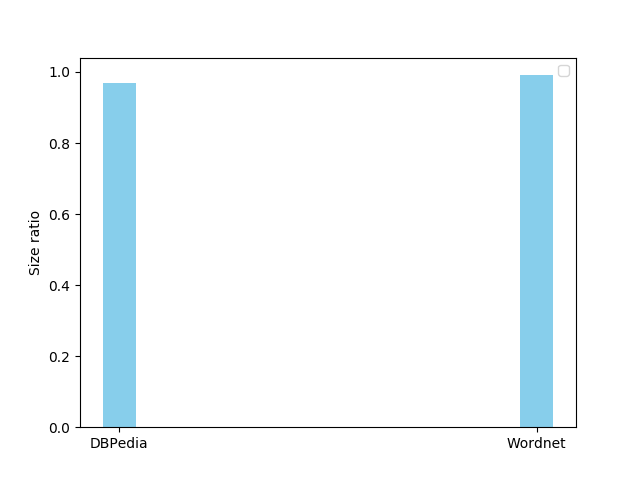
\includegraphics[width=0.5\textwidth]{figures/4_evaluation/ontology/sizeRatiosSymmetricsDelete}\label{fig:sizeratiossymmetricsdelete}}
	\caption{Results for deleting symmetric properties, on the grammar level (\ref{fig:edgeratiossymmetricsdelete}) and on the file size level (\ref{fig:sizeratiossymmetricsdelete}).}
	\label{fig:symmetricDeleteResults}
\end{figure}

The evaluation results are illustrated in Fig.~\ref{fig:symmetricAddResults2}. Of course, $IER>1$ is true and $IER$ is bigger than in Fig.~\ref{fig:edgeratiossymmetricsadd}, since now a higher amount of edges has been added. The fact that both $OER$~(Fig.~\ref{fig:edgeratiossymmetricsadd2}) and $SR$~(Fig.~\ref{fig:sizeratiossymmetricsadd2}) are lower than 1, support our hypothesis that adding symmetric edges is more beneficial than removing them.

\begin{figure}[h]
	\centering
	\subfloat[$IER$ and $OER$]{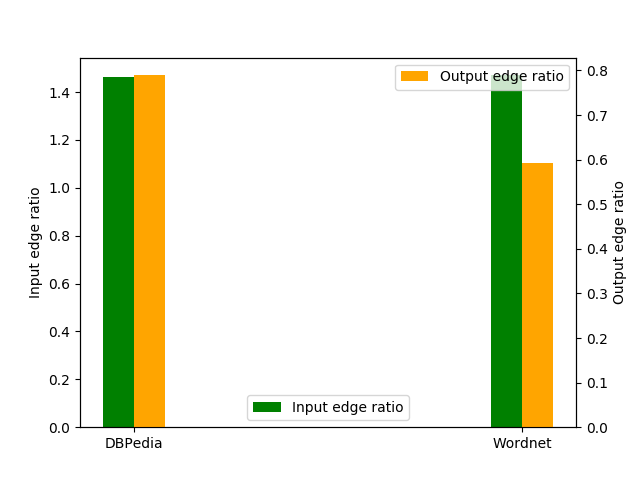
\includegraphics[width=0.5\textwidth]{figures/4_evaluation/ontology/edgeRatiosSymmetricsAdd2}\label{fig:edgeratiossymmetricsadd2}}
	\hfill 
	\subfloat[$SR$]{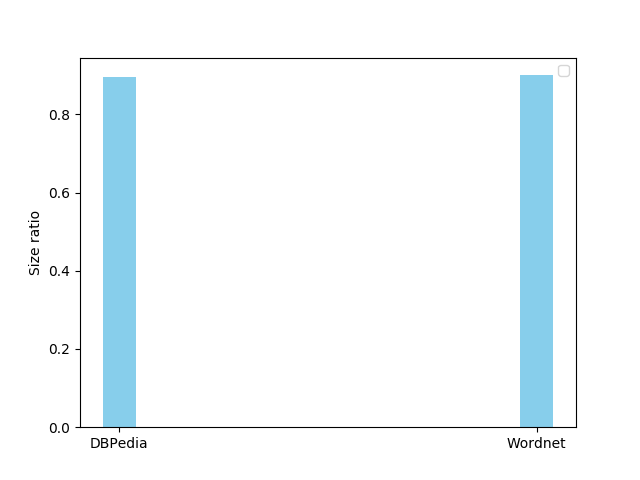
\includegraphics[width=0.5\textwidth]{figures/4_evaluation/ontology/sizeRatiosSymmetricsAdd2}\label{fig:sizeratiossymmetricsadd2}}
	\caption{Results for adding symmetric properties, on the grammar level (\ref{fig:edgeratiossymmetricsadd2}) and on the file size level (\ref{fig:sizeratiossymmetricsadd2}). In contrast to Fig.~\ref{fig:symmetricAddResults}, the input graph $in_1$ contains only one direction for each triple with a symmetric property.}
	\label{fig:symmetricAddResults2}
\end{figure}


\subsubsection{Inverse Properties}

\subsubsection{Transitive Properties}

\subsubsection{Everything Together}

\subsection{Dictionary Improvements}\label{sec:evaluationDictImprovements}

At this point  about the evaluation of the approaches from Ch.~\ref{sec:implementationDictImprovements}. First the Huffman compression of literals is evaluated and then the compression of blank node IDs. 


\subsubsection{Literals}

As already mentioned, a self-generated Huffman code was used to compress the literals of an RDF graph, as it is likely to get a better compression than the with the prefix-based compression of HDT.

Now the results of the evaluation are presented. First, the Semantic Web Dog Food data set is used. This is well suited for an evaluation, since both literals and URIS are included as objects. Fig.~\ref{fig:dogfoodcomprratios} shows $CR(out_{dict})$ for a subset of the data (DF0 - DF9). 


\begin{figure}
	\centering
	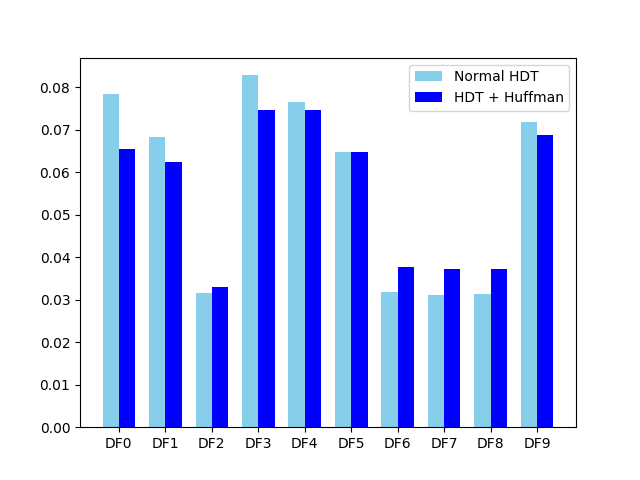
\includegraphics[width=0.7\linewidth]{figures/4_evaluation/dogFoodComprRatios}
	\caption{$CR(out_{dict})$. Comparison between Normal HDT and HDT + Huffman.}
	\label{fig:dogfoodcomprratios}
\end{figure}

It can be seen that the use of the Huffman code only brings a small improvement in some cases. In some cases Normal HDT even compresses better than HDT with Huffman.

This is because these data do not have a very high proportion of literals and literals are also rather short. This can be seen in Fig.~\ref{fig:dogfood}, where Fig.\ref{fig:dogfoodcomprratiosSub} lists $CR(out_{dict})$ again and Fig.\ref{fig:dogfoodliteralanalysis} shows the relative proportion of literals and the average length of a literal. The proportion of literals in the triples is never higher than 17.5\% and the highest average literal length is about 12. So these are single words rather than whole texts. Only in cases where both the proportion and the literal length are relatively high, an improvement can be seen (e.g. with DF9).


\begin{figure}[h]
	\centering
	\subfloat[$CR(out_{dict})$ for Normal HDT and HDT + Huffman]{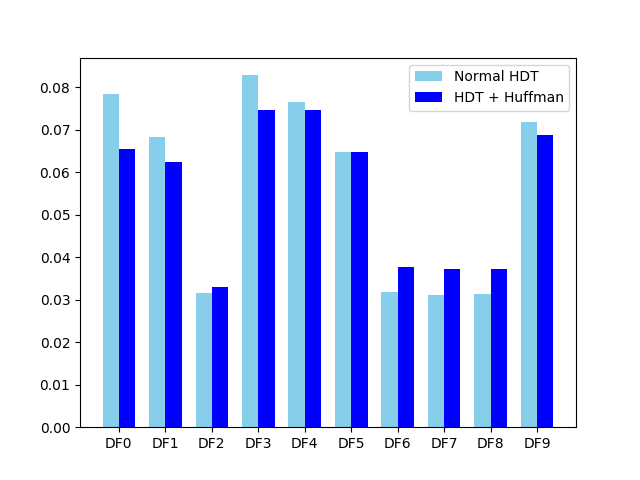
\includegraphics[width=0.5\textwidth]{figures/4_evaluation/dogFoodComprRatios}\label{fig:dogfoodcomprratiosSub}}
	\hfill
	\subfloat[Relative amounts of literals and average literal length.]{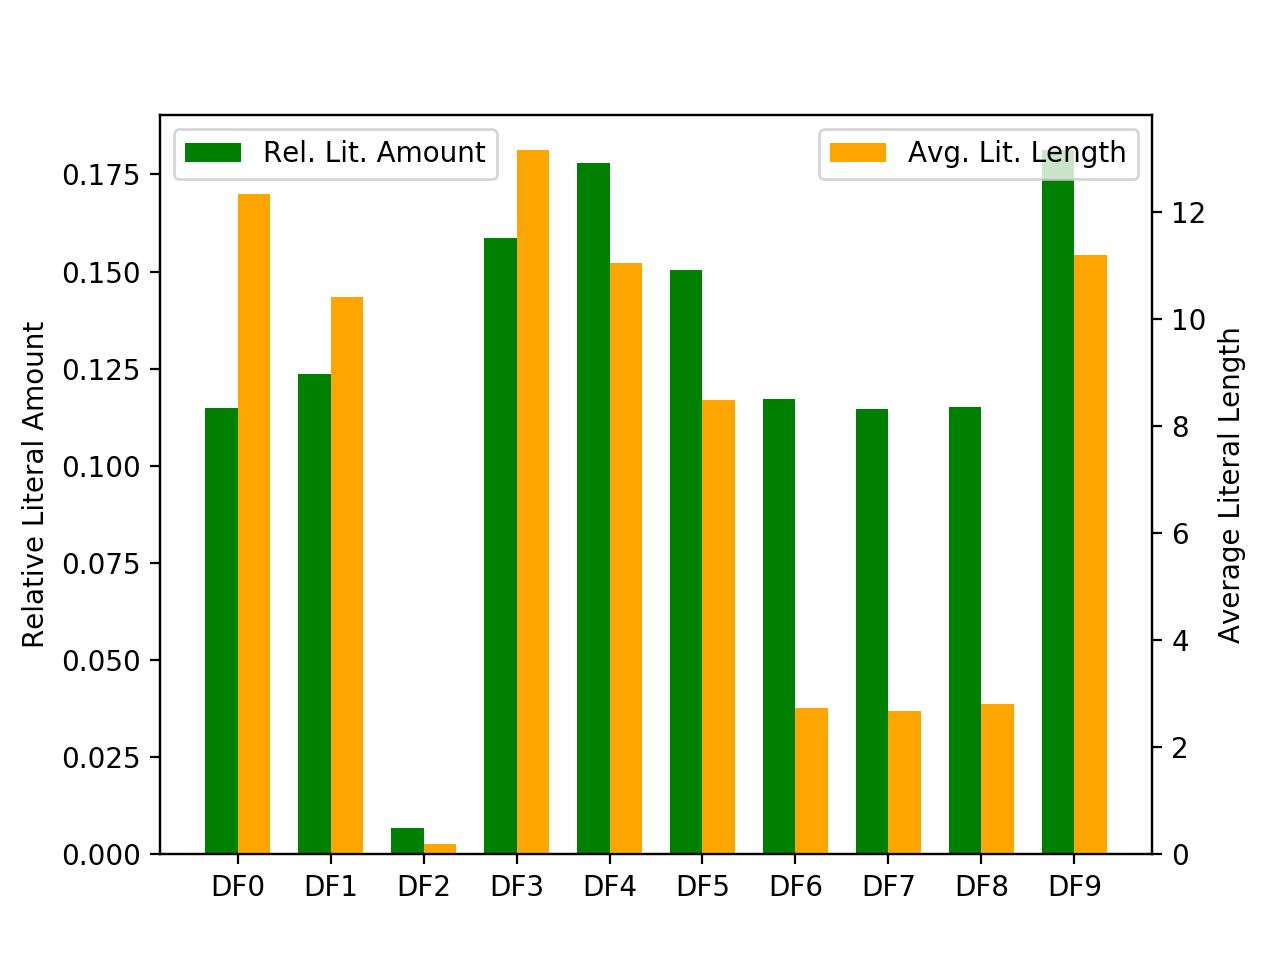
\includegraphics[width=0.5\textwidth]{figures/4_evaluation/dogFoodLiteralAnalysis}\label{fig:dogfoodliteralanalysis}}
	\caption{Relation between literal percentage and literal length (right) and $CR(out_{dict})$ (left) for Semantic Web Dog Food Data.}
	\label{fig:dogfood}
\end{figure}

Now the DBPedia data set is considered, because it has a different structure of data. Here, graphs are considered which contain the abstracts of Wikipedia, because these are longer texts. In addition there are abstracts in different languages, so it can be seen whether some languages are better suited for Huffman than others.

Fig.~\ref{fig:dbAbstractscomprratiosSub} shows $CR(out_{dict})$ for the abstract files. The abbreviations stand for the languages in which the abstracts are written. It can be seen that Huffman significantly improves $CR(out_{dict})$ here. The reason for this can be seen in Fig.~\ref{fig:dbAbstractsliteralanalysis}, where the average literal length is illustrated. The relative proportion of literals is not shown this time, since it is 100\% for all files. The average literal length varies between languages, but is generally much higher than in Semantic Web Dog Food. Therefore, the improvement is much greater here.

Another phenomenon can also be seen here: Although the English file contains by far the longest literals, the improvement by Huffman here is not as big as, for example, in the Bulgarian file. In the English case, the Huffman code is less effective because there are fewer different characters than in the other languages. Huffman is generally more efficient on large alphabets, according to~\cite{huffman}.

\begin{figure}[h]
	\centering
	\subfloat[$CR(out_{dict})$ for Normal HDT and HDT + Huffman]{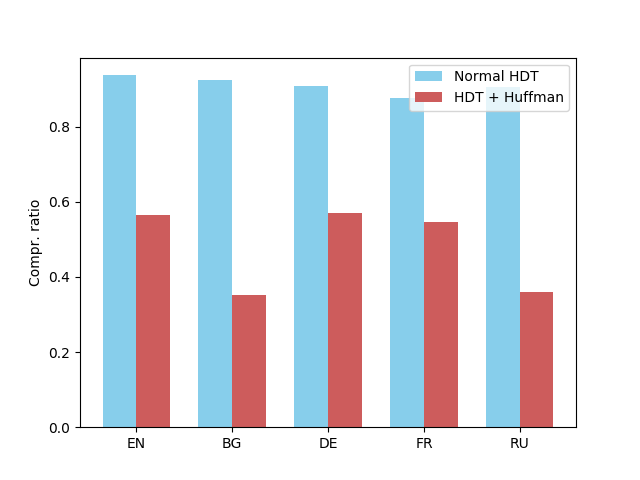
\includegraphics[width=0.5\textwidth]{figures/4_evaluation/dbAbstractsComprRatios}\label{fig:dbAbstractscomprratiosSub}}
	\hfill
	\subfloat[Average literal length.]{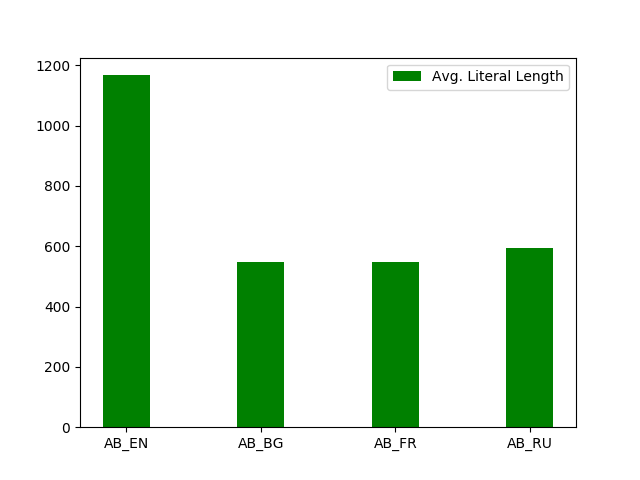
\includegraphics[width=0.5\textwidth]{figures/4_evaluation/dbAbstractsLiteralAnalysis}\label{fig:dbAbstractsliteralanalysis}}
	\caption{Relation between literal length (b) and compression ratios (a) for DBPedia Abstracts (Abbreviations denote the languages the abstracts are written in).}
	\label{fig:dbAbstracts}
\end{figure}

As mentioned above, saving the Huffman code means almost no additional storage effort. The average fraction of the Huffman code is about 0.1\% and was therefore not displayed in the visualizations.

Since the calculation of the Huffman code increases the runtime of the whole compression, it is now considered how big this effect is. Fig.~\ref{fig:dbAbstractsRuntimes} shows $CT$ for the compression of the DBPedia abstract data. Here, $CT$ has been increased very much. This is because HDT can normally compress very little with this data because of the many long literals and is therefore finished quite quickly. With Huffman the data can be compressed much better and it takes quite a long time.

Fig.~\ref{fig:dogFoodRuntimes} shows $CT$ for the Semantic Web Dog Food data, where the run times are only slightly longer, because Huffman hardly improves the compression.

So it can be said that the use of a standard Huffman code could be worthwhile because of the otherwise high runtime. At this point, however, the evaluation with such a standard code was omitted, since such existing codes do not contain all the special characters that occur in RDF data.


\begin{figure}[h]
	\centering
	\subfloat[$CT$ for DBPedia abstracts.]{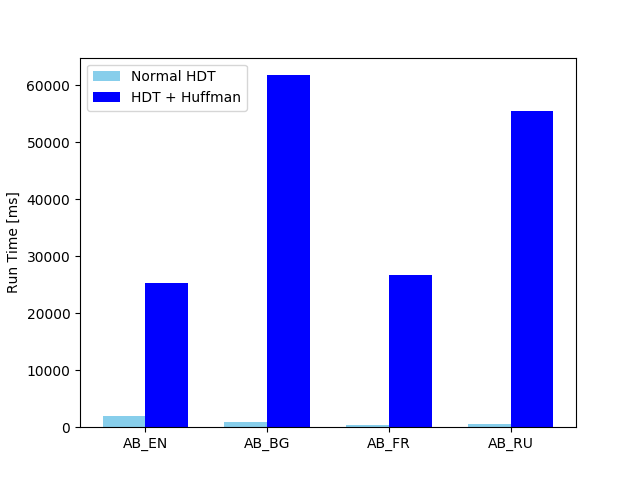
\includegraphics[width=0.5\textwidth]{figures/4_evaluation/dbAbstractsRuntimes}\label{fig:dbAbstractsRuntimes}}
	\hfill
	\subfloat[$CT$ for Semantic Web Dog Food files.]{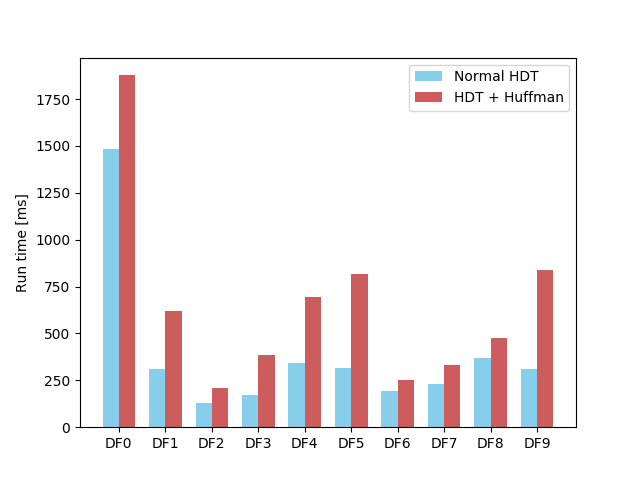
\includegraphics[width=0.5\textwidth]{figures/4_evaluation/dogFoodRuntimes}\label{fig:dogFoodRuntimes}}
	\caption{Run times ($CT$) for Normal HDT and HDT + Huffman.}
	\label{fig:huffmanRuntimes}
\end{figure}

\subsubsection{Blank Nodes}

\subsection{Ontology and Dictionary}
\todo{evtl beides anwenden,wahrscheinl. ist ont Anteil so gering dass man es auf Grafik nicht sehen kann}






























